El sistema de control de accesos de SMARTEST esta formado por tres subsistemas funcionales intimamente relacionados:

\begin{itemize}
\item El servidor de base de datos.- Los datos de usuario son administrados a través de una aplicación web, la cual tiene un API Json que da servicio a la consulta de usuarios.
\item El APP de usuario.- Es una APP de celular que genera los códigos QR de acceso al usuario una vez que ingresa su clave y contraseña.
\item El dispositivo de acceso.- Esta formado por dos lectores, uno de entrada y otro de salida, un torniquete o puerta de control, y una pantalla o semáforo para indicar que el acceso fue permitido o negado
\end{itemize}

\begin{figure}[htb]
\centering
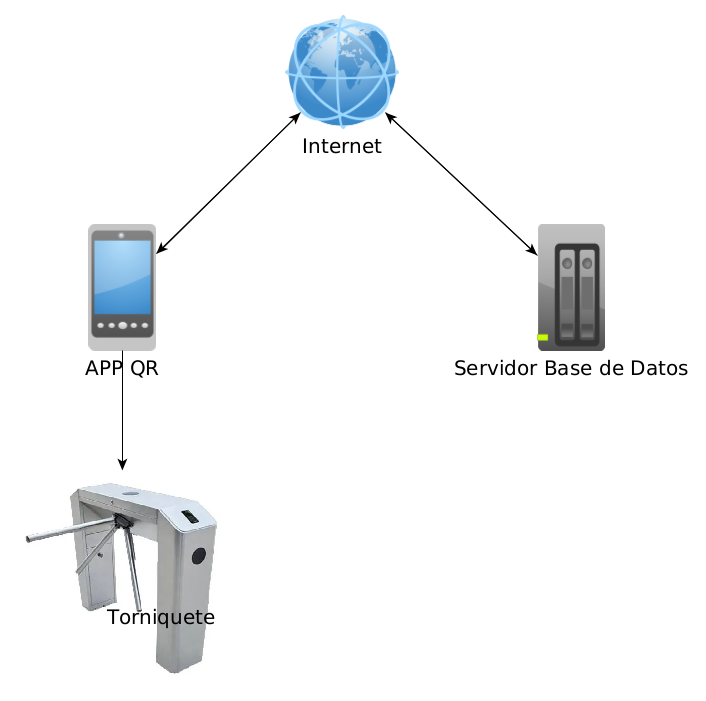
\includegraphics[width=0.4\textwidth]{capitulo1/sistema_acceso.png}
\caption{Sistema de Acceso SMARTEST}
\label{cap1:001}
\end{figure}
